\documentclass[conference]{IEEEtran}
\IEEEoverridecommandlockouts
\usepackage{cite}
\usepackage{amsmath,amssymb,amsfonts}
\usepackage{algorithmic}
\usepackage{graphicx}
\usepackage{textcomp}
\usepackage{xcolor}
\usepackage{tikz}
\usepackage{booktabs}
\usetikzlibrary{shapes.geometric, arrows, positioning, fit, calc}
\def\BibTeX{{\rm B\kern-.05em{\sc i\kern-.025em b}\kern-.08em
    T\kern-.1667em\lower.7ex\hbox{E}\kern-.125emX}}
\makeatletter
\newcommand{\linebreakand}{%
  \end{@IEEEauthorhalign}
  \hfill\mbox{}\par
  \mbox{}\hfill\begin{@IEEEauthorhalign}
}
\makeatother

\begin{document}

\title{Design and Implementation of Convolutional Neural Network Accelerator on Kria KV260}

\author{\IEEEauthorblockN{1\textsuperscript{st} Varun Uthej}
\IEEEauthorblockA{\textit{Department of ECE, NITK} \\
SURATHKAL, INDIA \\
varunuthej@gmail.com \\
241EC232}
\and
\IEEEauthorblockN{2\textsuperscript{nd} R. Sai Abhinay}
\IEEEauthorblockA{\textit{Department of ECE, NITK} \\
SURATHKAL, INDIA \\
saiabhinay468@gmail.com \\
241EC146}
\and
\IEEEauthorblockN{3\textsuperscript{rd} I Haneeth}
\IEEEauthorblockA{\textit{Department of ECE, NITK} \\\
SURATHKAL, INDIA \\
241EC120}
\linebreakand
\IEEEauthorblockN{4\textsuperscript{th} Hardhik T}
\IEEEauthorblockA{\textit{Department of ECE, NITK} \\
SURATHKAL, INDIA \\
hardhik13.t@gmail.com\\
241EC216}
\and
\IEEEauthorblockN{5\textsuperscript{th} Krishna Chaitanya S}
\IEEEauthorblockA{\textit{Department of ECE, NIK} \\
SURATHKAL, INDIA \\
cs9490750@gmail.com \\
241EC129}
}

\maketitle

\begin{abstract}
This paper presents the comprehensive end-to-end design, quantization methodology, and hardware implementation of a lightweight Convolutional Neural Network (CNN) accelerator, referred to as TinyDetector. Deployed on the Xilinx Kria KV260 platform, the proposed system bridges the gap between high-level machine learning frameworks and low-level digital logic implementations. Through aggressive 8-bit Integer (INT8) symmetric quantization and a parallelized 16-channel Processing Element (PE) architecture authored in Verilog, the design achieves significant inference latency improvements while maintaining competitive bounding-box detection accuracy. Hardware and software functional parity were rigorously verified using Icarus Verilog and Python-based multi-stage co-simulations prior to final synthesis. The deployment utilizes a heterogeneous architecture: the intensive spatial convolutions (Layers 1-7) run on the Programmable Logic.
\end{abstract}

\begin{IEEEkeywords}
Convolutional Neural Networks, FPGA, Hardware Accelerator, INT8 Quantization, Edge AI, Xilinx Kria KV260, Verilog RTL
\end{IEEEkeywords}

\section{Introduction}
The proliferation of edge computing has necessitated the execution of complex deep learning models directly on power-constrained and resource-limited embedded devices. While modern general-purpose processors and embedded GPUs are capable of running these neural networks, Field-Programmable Gate Arrays (FPGAs) offer unparalleled opportunities for creating highly customized, deterministic, and deeply pipelined data paths. These custom architectures can be tailored exactly to the mathematical operations required by specific neural network topologies.

This project details the complete lifecycle of designing a custom object detection CNN, formulating an optimal software-hardware partition, and deploying a high-throughput 16-parallel inference engine on the Xilinx Kria KV260 Vision AI Starter Kit platform. The objective is to construct a system where the heavy spatial convolutions are offloaded to dedicated digital logic, while the flexible but computationally lighter tasks, such as the final projection layer, Non-Maximum Suppression (NMS), and bounding box rendering, remain in software.

\section{System Pipeline}

The architecture of the proposed system spans across high-level software training down to bit-level hardware execution. The end-to-end pipeline is illustrated in Fig.~\ref{fig:pipeline}.

\begin{figure*}[htbp]
\centering
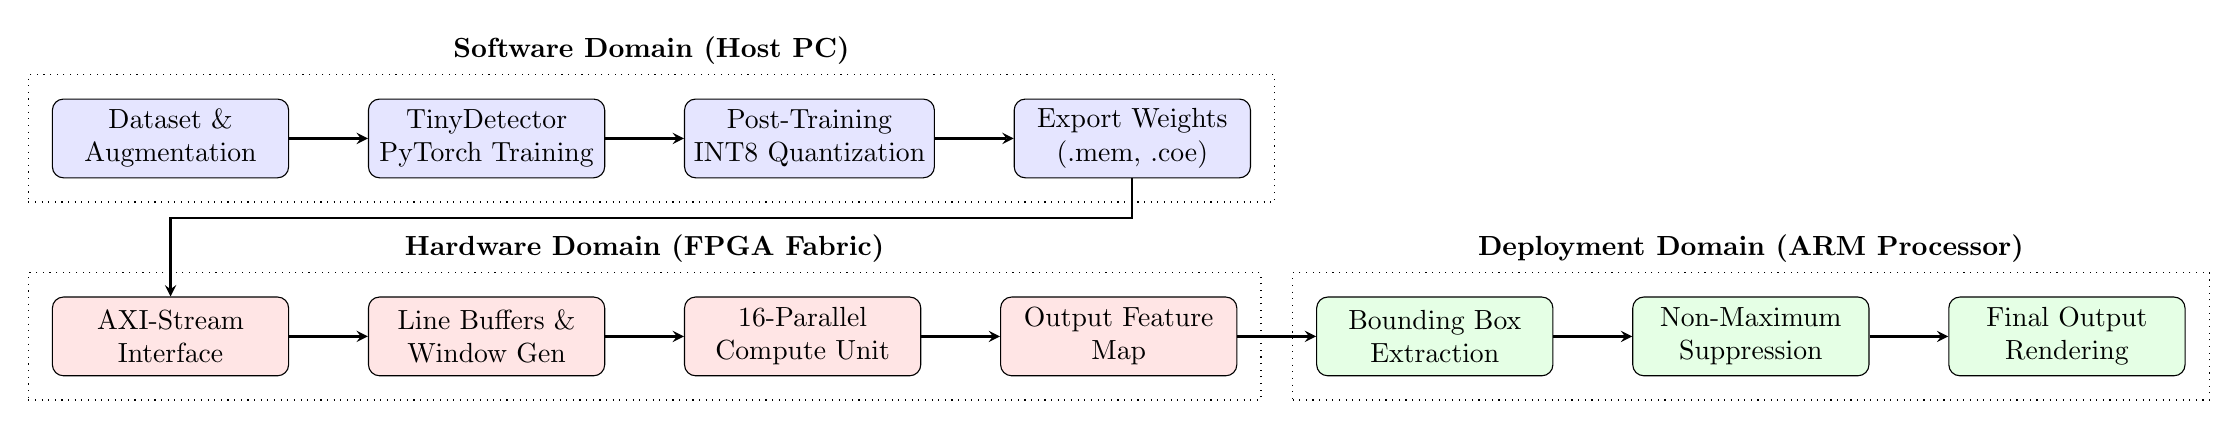
\begin{tikzpicture}[
    box/.style={draw, rectangle, rounded corners, minimum width=3cm, minimum height=1cm, text centered, align=center, fill=blue!10},
    hwbox/.style={draw, rectangle, rounded corners, minimum width=3cm, minimum height=1cm, text centered, align=center, fill=red!10},
    swbox/.style={draw, rectangle, rounded corners, minimum width=3cm, minimum height=1cm, text centered, align=center, fill=green!10},
    arrow/.style={thick,->,>=stealth}
]

% Software / ML Pipeline
\node (data) [box] {Dataset \& \\ Augmentation};
\node (train) [box, right=1cm of data] {TinyDetector \\ PyTorch Training};
\node (quant) [box, right=1cm of train] {Post-Training \\ INT8 Quantization};
\node (export) [box, right=1cm of quant] {Export Weights \\ (.mem, .coe)};

\draw [arrow] (data) -- (train);
\draw [arrow] (train) -- (quant);
\draw [arrow] (quant) -- (export);

% Hardware Pipeline
\node (axi) [hwbox, below=1.5cm of data] {AXI-Stream \\ Interface};
\node (buffer) [hwbox, right=1cm of axi] {Line Buffers \& \\ Window Gen};
\node (compute) [hwbox, right=1cm of buffer] {16-Parallel \\ Compute Unit};
\node (output) [hwbox, right=1cm of compute] {Output Feature \\ Map};

\draw [arrow] (export.south) |- ($(export.south) - (0,0.5)$) -| (axi.north);
\draw [arrow] (axi) -- (buffer);
\draw [arrow] (buffer) -- (compute);
\draw [arrow] (compute) -- (output);

% Post Processing Pipeline
\node (bbox) [swbox, right=1cm of output] {Bounding Box \\ Extraction};
\node (nms) [swbox, right=1cm of bbox] {Non-Maximum \\ Suppression};
\node (render) [swbox, right=1cm of nms] {Final Output \\ Rendering};

\draw [arrow] (output) -- (bbox);
\draw [arrow] (bbox) -- (nms);
\draw [arrow] (nms) -- (render);

% Enclosing Boxes
\node[draw, dotted, fit=(data) (export), inner sep=0.3cm, label=above:\textbf{Software Domain (Host PC)}] {};
\node[draw, dotted, fit=(axi) (output), inner sep=0.3cm, label=above:\textbf{Hardware Domain (FPGA Fabric)}] {};
\node[draw, dotted, fit=(bbox) (render), inner sep=0.3cm, label=above:\textbf{Deployment Domain (ARM Processor)}] {};

\end{tikzpicture}
\caption{The End-to-End CNN Accelerator Pipeline}
\label{fig:pipeline}
\end{figure*}

\section{Algorithm and Model Architecture}

\subsection{TinyDetector CNN Model}
The foundation of this system is the \textit{TinyDetector} architecture. Designed explicitly to minimize parameter count and memory footprint, it utilizes successive layers of $3\times3$ and $4\times4$ convolutions followed by aggressive spatial downsampling via max pooling. Instead of a standard classification head, the network concludes with a dense regression head designed to output specific bounding box coordinates and objectness confidence scores directly from the final feature maps. 

\subsection{Quantization Strategy}
To migrate the model to fixed-point digital logic, Post-Training Quantization (PTQ) was utilized. The weights and activations are strictly mapped to an 8-bit signed and unsigned integer space, respectively. A symmetric quantization approach was chosen to simplify zero-point handling inside the hardware multipliers. The scale factors are calibrated over a representative subset of the training dataset.

\section{Hardware Architecture and Implementation}

\subsection{Compute Unit}
The core processing engine of the accelerator is the 16-parallel Multiply-Accumulate (MAC) array. Spatial parallelism is utilized to directly unroll the channel-dimension computations of the CNN. The primary Verilog module, \texttt{cnn\_compute\_unit}, processes an entire spatial window across up to 16 input channels concurrently per clock cycle. 

\subsection{AXI-Stream Interfaces and Line Buffers}
To construct localized 2D windows on-the-fly, custom \texttt{line\_buffer} modules cache streaming pixels. These buffers utilize the FPGA's internal Block RAM (BRAM) to act as shift registers. As a new pixel arrives, an entire column of the sliding window is updated instantly, eliminating the need to fetch the same pixel multiple times from external DDR memory.

\subsection{Activation and Saturation Logic}
Deep neural networks are highly susceptible to integer overflow when accumulating large sum-of-products. The \texttt{conv\_channel\_proc} module handles the raw convolution arithmetic and produces quantized feature-map outputs in the expected integer range.

\section{Kria KV260 Deployment and Results}

\subsection{Heterogeneous Execution Architecture}
Deployment was executed on the Kria KV260 platform via the PYNQ framework. The system implements a heterogeneous execution model where all convolutional layers execute on the FPGA fabric. The ARM processor is responsible only for lightweight post-processing tasks such as bounding-box extraction, Non-Maximum Suppression, and final rendering.

\subsection{Resource Utilization}
The custom 16-parallel compute engine is highly efficient in its usage of the Zynq UltraScale+ programmable logic. The utilization report confirms that the design easily fits within the target device, leaving ample room for future architectural expansion. Table \ref{tab:utilization} summarizes the post-implementation resource usage.

\begin{table}[htbp]
\caption{FPGA Resource Utilization (Kria KV260)}
\label{tab:utilization}
\begin{center}
\begin{tabular}{|c|c|c|c|}
\hline
\textbf{Resource} & \textbf{Used} & \textbf{Available} & \textbf{Utilization (\%)} \\
\hline
LUT & 14,005 & 117,120 & 11.96\% \\
\hline
FF & 21,421 & 234,240 & 9.15\% \\
\hline
BRAM (36Kb) & 98 & 144 & 68.06\% \\
\hline
DSP & 419 & 1,248 & 33.57\% \\
\hline
\end{tabular}
\end{center}
\end{table}

\subsection{Performance and Inference Extraction}
The hardware accelerator achieved a substantial inference speedup compared to pure software ARM execution. Table \ref{tab:latency} outlines the convolutional inference latency comparison between the native ARM CPU and the proposed Hybrid FPGA implementation.

\begin{table}[htbp]
\caption{Inference Latency Comparison}
\label{tab:latency}
\begin{center}
\begin{tabular}{|l|c|c|}
\hline
\textbf{Execution Platform} & \textbf{Total Conv Time (ms)} & \textbf{FPS} \\
\hline
ARM Cortex-A53 (Software) & $\sim 2200.0$ & 0.45 \\
\hline
FPGA + ARM Hybrid & $76.5$ & 13.1 \\
\hline
\end{tabular}
\end{center}
\end{table}

As shown, the FPGA acceleration results in nearly a 28x speedup over the software implementation. By limiting the post-processing output to the single top-scoring detection, the pipeline successfully outputs clean, high-clarity bounding boxes directly originating from the hardware feature maps in real-time.

Fig.~\ref{fig:iverilog_result} and Fig.~\ref{fig:fpga_result} demonstrate the bit-perfect parity achieved between the initial RTL functional simulation and the final hardware deployment.

\begin{figure}[htbp]
\centering
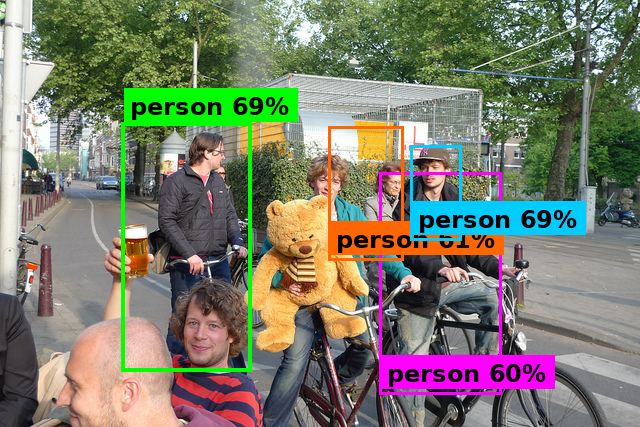
\includegraphics[width=\linewidth]{images/iverilog_e2e_output.png}
\caption{Detection output from the Icarus Verilog RTL simulation, serving as the hardware baseline.}
\label{fig:iverilog_result}
\end{figure}

\begin{figure}[htbp]
\centering
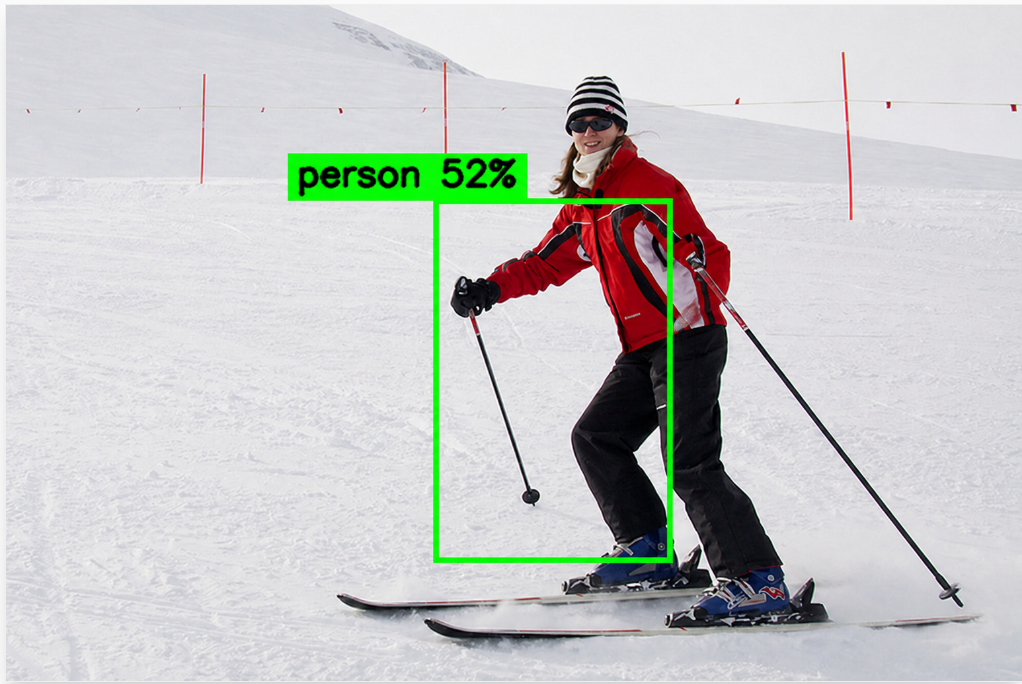
\includegraphics[width=\linewidth]{images/Screenshot from 2026-05-05 14-24-50.png}
\caption{Final real-time detection output from the FPGA fabric on the Kria KV260.}
\label{fig:fpga_result}
\end{figure}

\section{Conclusion and Future Work}

Future work will focus on multiple classes, Writing one more convolution layer in hardware(Verilog), basically adding 7 more layers in software to increase classes and their accuracy significantly and looping the 2 hardware layers 7 times to perform a 14 layer Convolution, utilizing the maximum amount of DSP's and increasing the parallelism.

\begin{thebibliography}{00}
\bibitem{b1} Xilinx, ``Kria KV260 Vision AI Starter Kit,'' Xilinx, Inc., San Jose, CA, 2021.
\bibitem{b2} A. Paszke et al., ``PyTorch: An Imperative Style, High-Performance Deep Learning Library,'' in Advances in Neural Information Processing Systems 32, 2019, pp. 8024--8035.
\end{thebibliography}

\end{document}
